\documentclass[aspectratio=169,11pt]{beamer}
\usepackage[utf8]{inputenc}
\usepackage[T1]{fontenc}
\usepackage[spanish]{babel}
\usepackage{amsmath,amssymb}
\usepackage{tikz}
\usetikzlibrary{arrows.meta,angles,calc,positioning}
\usetheme{Madrid}
\usecolortheme{default}
\setbeamertemplate{navigation symbols}{}
\setbeamertemplate{blocks}[rounded][shadow=false]
\newcommand{\ang}[1]{\angle #1^\circ}

\title[Especificaciones y bounds]{Paso 8: Especificaciones y bounds}
\subtitle{Convertir lo que se exige al lazo cerrado en zonas prohibidas del Nichols}
\author{Curso de control robusto (QFT)}
\date{}
\begin{document}
\begin{frame}\titlepage\end{frame}

\begin{frame}{Dónde encaja este paso}
  \tiny
  \begin{enumerate}\setlength{\itemsep}{-2pt}
    \item[1.] Números complejos \hfill \textcolor{gray}{(hecho)}
    \item[2.] Funciones de transferencia: $s$, polos y ceros \hfill \textcolor{gray}{(hecho)}
    \item[3.] Respuesta en frecuencia: $s=j\omega$, magnitud y fase \hfill \textcolor{gray}{(hecho)}
    \item[4.] Decibelios y escala logarítmica (Bode) \hfill \textcolor{gray}{(hecho)}
    \item[5.] Realimentación: $L$, $T=\frac{L}{1+L}$, $S=\frac{1}{1+L}$ \hfill \textcolor{gray}{(hecho)}
    \item[6.] Nichols chart \hfill \textcolor{gray}{(hecho)}
    \item[7.] Incertidumbre y templates \hfill \textcolor{gray}{(hecho)}
    \item[\textbf{8.}] \textbf{Especificaciones $\rightarrow$ bounds} \hfill $\leftarrow$ estamos aquí
    \item[9.] Loop shaping, prefiltro y verificación
    \item[10.] QFT en control digital
    \item[11.] Dos caminos digitales: $z$ y $w$
    \item[12.] Estabilidad, límites, más especificaciones y caso real
    \item[13.] Muestreo por eventos con periodo base $T$
    \item[14.] Sistemas de dos estados: lazo interno y externo
    \item[15.] QFT y sistemas no lineales
    \item[16.] Algoritmos de QFT: cómo funcionan por dentro
    \item[17.] QFT en Python: una biblioteca paso a paso
    \item[18.] QFT en MATLAB: el mismo código, otra sintaxis
    \item[19.] Historia, panorama y bibliografía
  \end{enumerate}
  \vspace{2pt}
  \begin{block}{Objetivo de hoy}
    Traducir las especificaciones (estabilidad, seguimiento, perturbación) en una curva por frecuencia, el \textbf{bound}, que separa dónde \emph{puede} y dónde \emph{no puede} estar el nominal $L_0(j\omega)$.
  \end{block}
\end{frame}

\begin{frame}{Qué se exige al lazo cerrado: tres especificaciones}
  \small
  Todas deben cumplirse para \textbf{todas} las plantas $P_i\in\mathcal{P}$, con $L_i=GP_i$:
  \begin{block}{1. Estabilidad robusta (margen)}
    $\displaystyle\left|\frac{L_i}{1+L_i}\right|\le W_s=1.2\ (1.58\text{ dB})$ para todo $\omega$: evita picos de resonancia.
  \end{block}
  \begin{block}{2. Seguimiento}
    $|T_L(j\omega)|\le|F\,T_i(j\omega)|\le|T_U(j\omega)|$: la respuesta, con el prefiltro $F$, queda dentro de una banda entre un modelo lento y uno rápido.
  \end{block}
  \begin{block}{3. Rechazo de perturbación en la salida}
    $\displaystyle|S_i|=\frac{1}{|1+L_i|}\le W_d(\omega)$: en $\omega\le0.5$, $W_d=0.3$ ($-10.5$ dB); en $0.5<\omega\le1$, $W_d=0.5$ ($-6$ dB).
  \end{block}
\end{frame}

\begin{frame}{Especificación 1: el óvalo prohibido}
  \small
  Del paso 6: $|T|=1.58$ dB es un contorno cerrado alrededor del punto crítico $(-180^\circ,\ 0\text{ dB})$.
  \begin{itemize}
    \item $|T_i|\le1.58$ dB significa: el punto $L_i$ debe estar \textbf{fuera} de ese óvalo.
    \item Con incertidumbre, \textbf{todos} los puntos del template trasladado deben estar fuera a la vez.
  \end{itemize}
  \begin{block}{Qué cambia respecto a una sola planta}
    Con una planta, basta que $L_0$ esté fuera del óvalo. Con un template de tamaño finito, el nominal tiene que estar \emph{más lejos}, lo suficiente para que ni siquiera la esquina más cercana toque el óvalo.
  \end{block}
\end{frame}

\begin{frame}{Deslizar el template: cómo aparece el bound ($\omega=2$)}
  \footnotesize
  \centering
  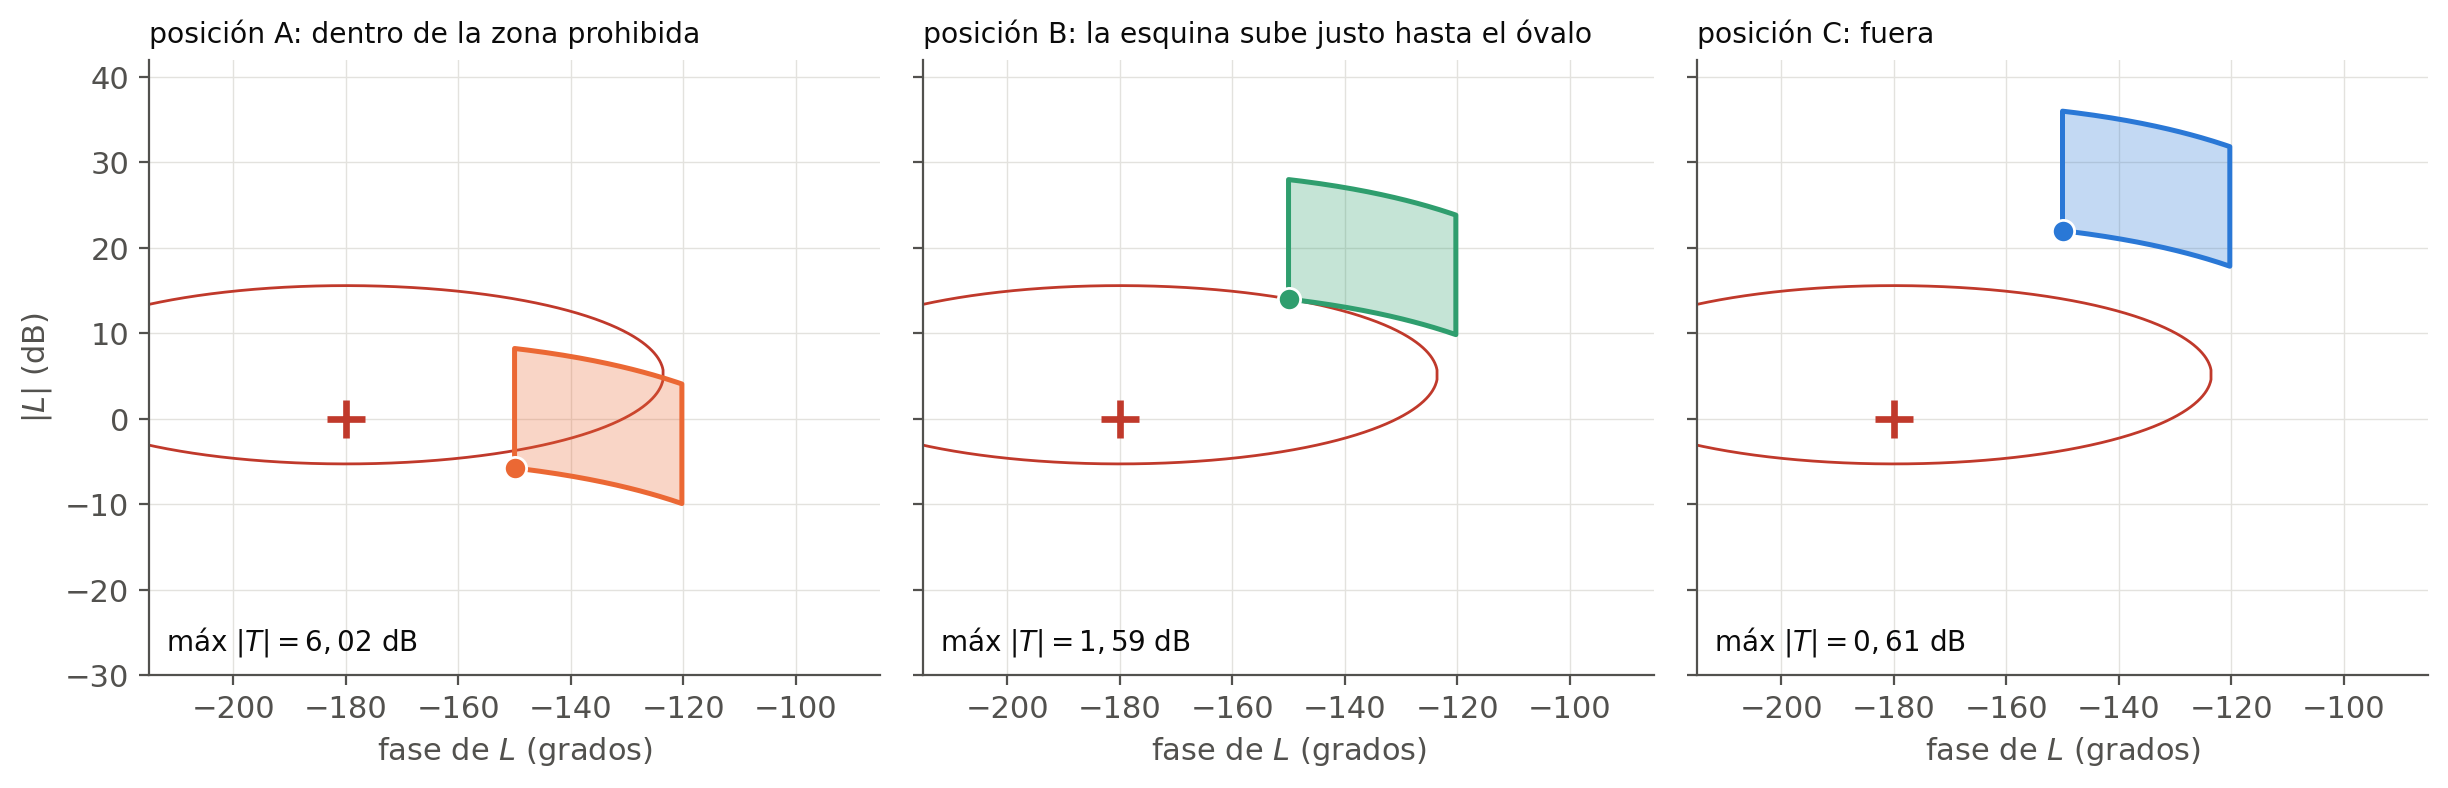
\includegraphics[width=\textwidth]{fig/deslizar.png}\\[2pt]
  Se mueve el nominal verticalmente a fase $-150^\circ$. En A el template se mete en el óvalo (máx $|T|=6.0$ dB); en B la esquina toca el borde ($1.58$ dB); en C todo queda fuera ($0.6$ dB). \textbf{B es un punto del bound.}
\end{frame}

\begin{frame}{Algoritmo: cómo se calcula un bound}
  \small
  \begin{block}{Para cada frecuencia $\omega_i$}
    \begin{enumerate}
      \item Calcular los cocientes $P_k(j\omega_i)/P_0(j\omega_i)$ de toda la familia: es la forma del template relativa al nominal.
      \item Recorrer una cuadrícula de posiciones del nominal: $(\varphi,g)$, es decir $L_0=10^{g/20}\angle\varphi$.
      \item En cada posición, formar $L_k=L_0\cdot\frac{P_k}{P_0}$ y comprobar las tres especificaciones para todos los $k$.
      \item Marcar la posición como permitida o prohibida.
      \item El \textbf{bound} es el borde entre las dos zonas.
    \end{enumerate}
  \end{block}
  \begin{alertblock}{Es mecánico}
    Se puede hacer con una hoja de cálculo o con unas pocas líneas de código. Lo difícil no es el cálculo sino interpretar el resultado.
  \end{alertblock}
\end{frame}

\begin{frame}{Seguimiento: la banda y cuánta variación se tolera}
  \footnotesize
  \centering
  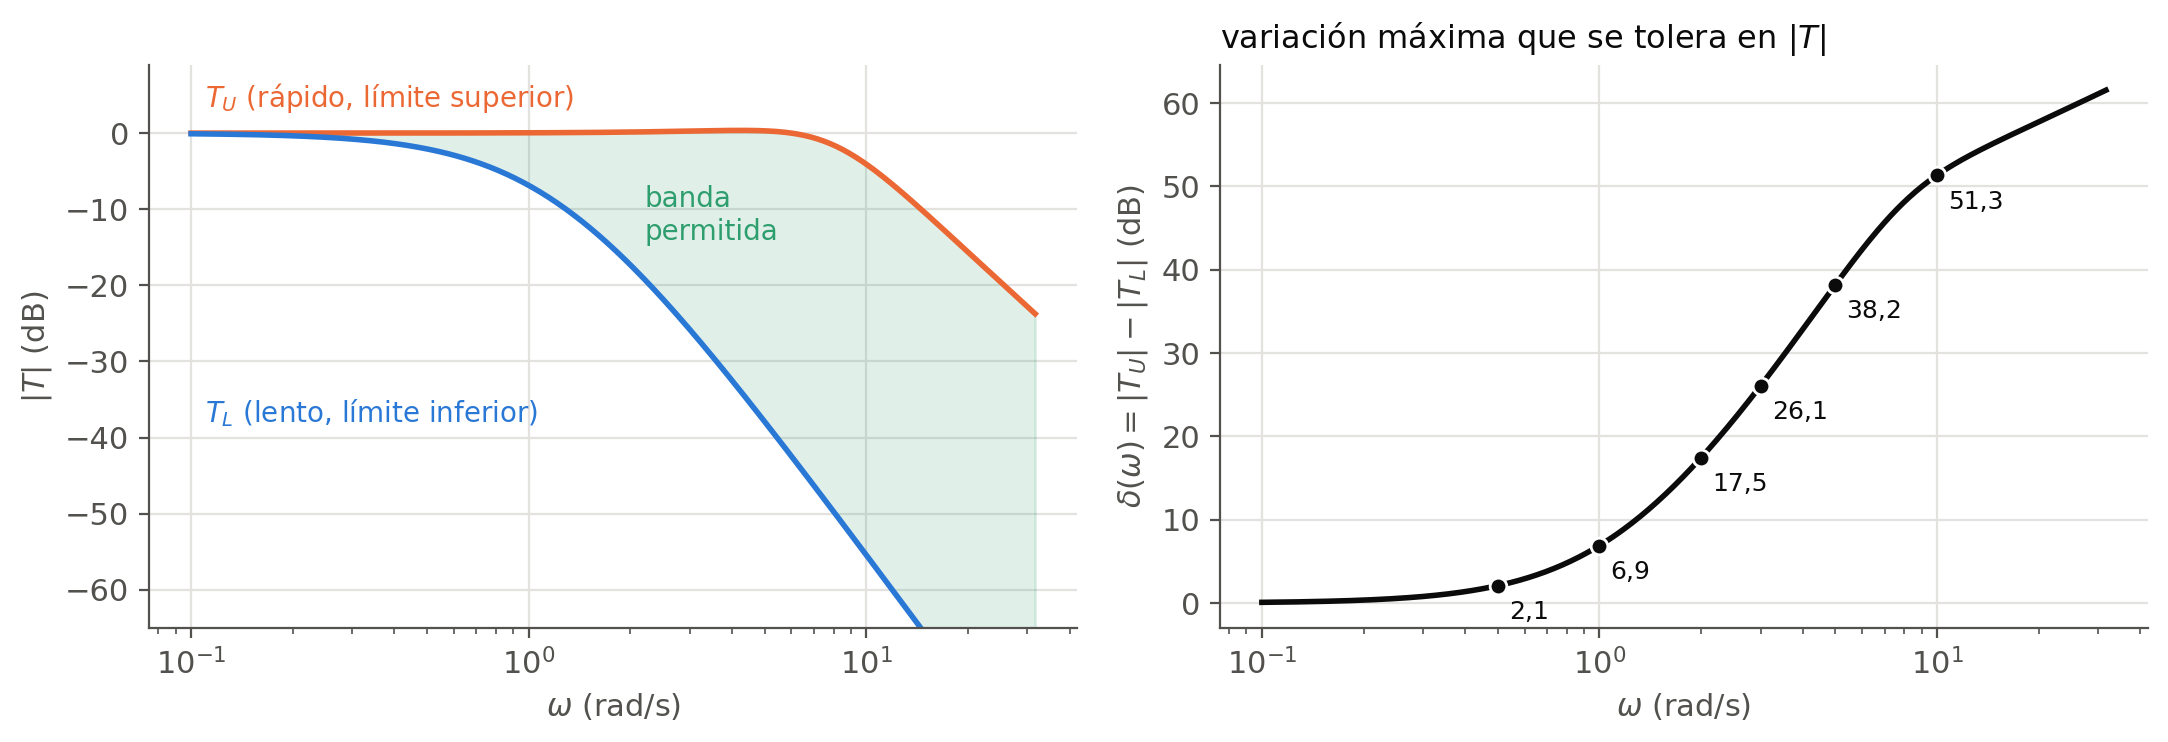
\includegraphics[width=\textwidth]{fig/banda.png}\\[2pt]
  \begin{columns}[T]
  \begin{column}{0.48\textwidth}
    $T_U$: segundo orden, $\omega_n=8$, $\zeta=0.6$. $T_L$: tres polos en $s=-1.2$.
  \end{column}
  \begin{column}{0.48\textwidth}
    $F$ es libre (paso 9), así que ahora solo importa la \emph{variación}: $\ \dfrac{\max_i|T_i|}{\min_i|T_i|}\le\dfrac{|T_U|}{|T_L|}=\delta(\omega)$.
  \end{column}
  \end{columns}
\end{frame}

\begin{frame}{Un mapa de posiciones permitidas ($\omega=1$)}
  \footnotesize
  \centering
  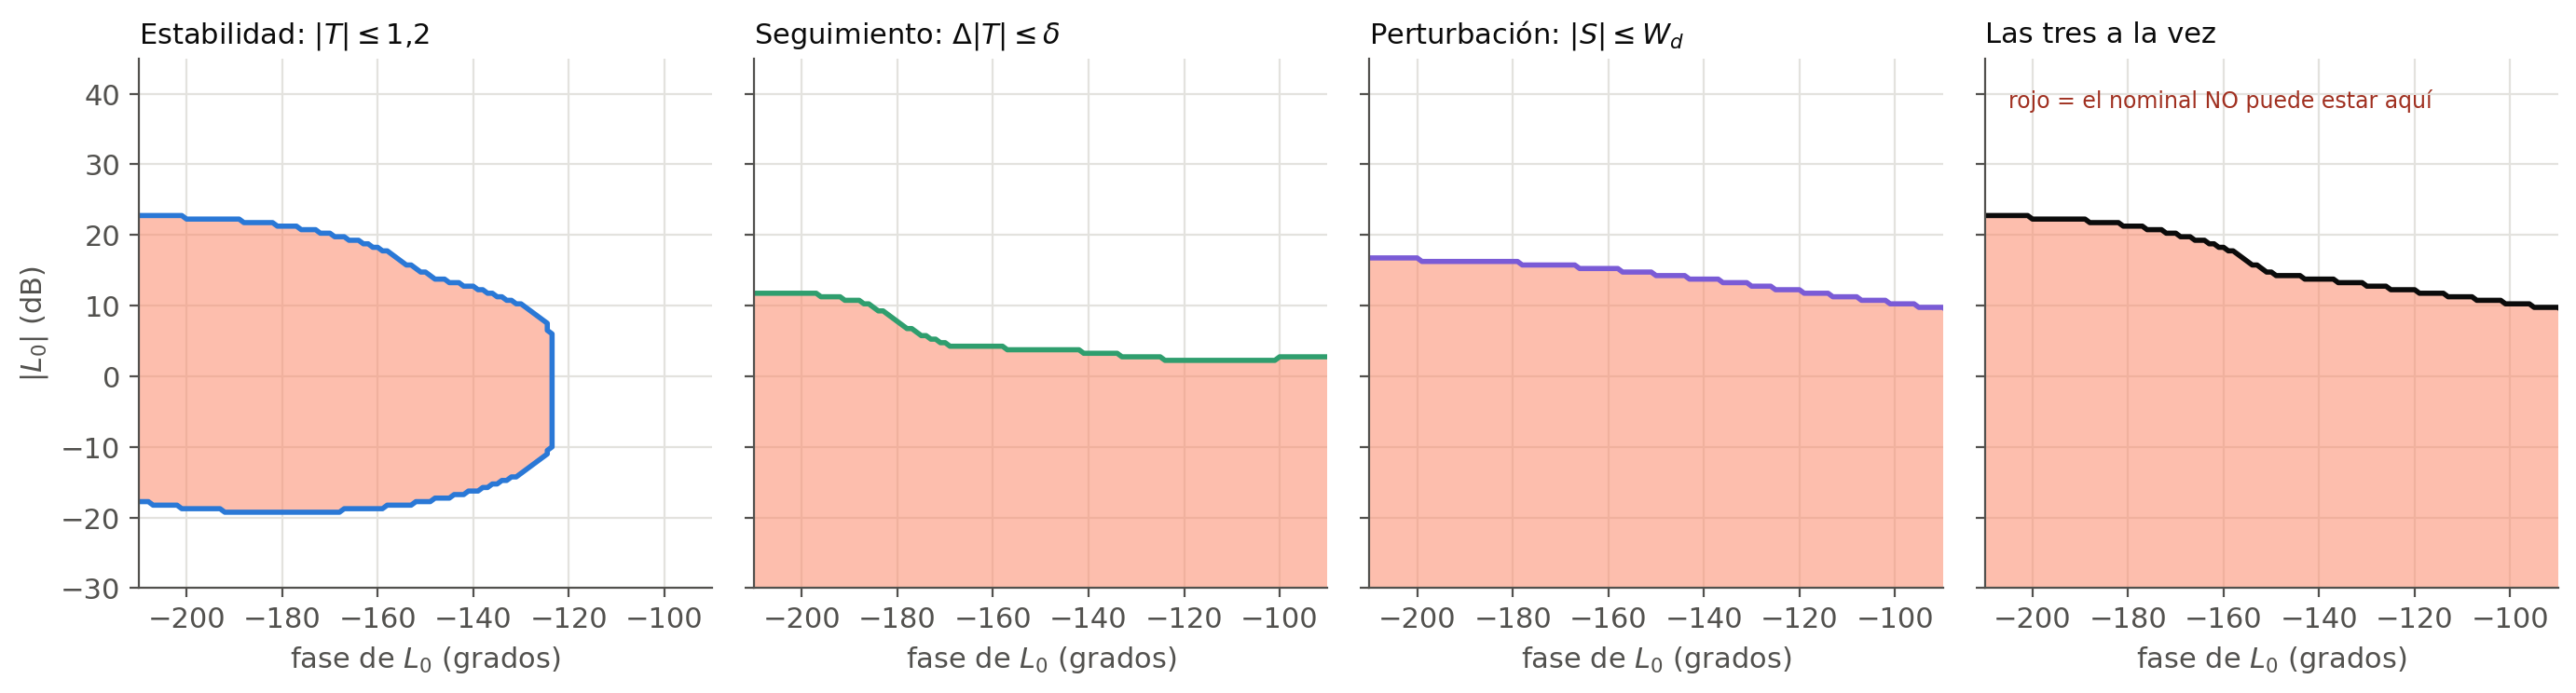
\includegraphics[width=\textwidth]{fig/mapas_w1.png}\\[2pt]
  \begin{columns}[T]
  \begin{column}{0.48\textwidth}
    Cada panel pinta de rojo las posiciones del nominal que \textbf{incumplen} esa especificación.
  \end{column}
  \begin{column}{0.48\textwidth}
    El bound final (derecha) es la unión: en cada fase manda la especificación más exigente.
  \end{column}
  \end{columns}
\end{frame}

\begin{frame}{Los bounds de todas las frecuencias}
  \footnotesize
  \centering
  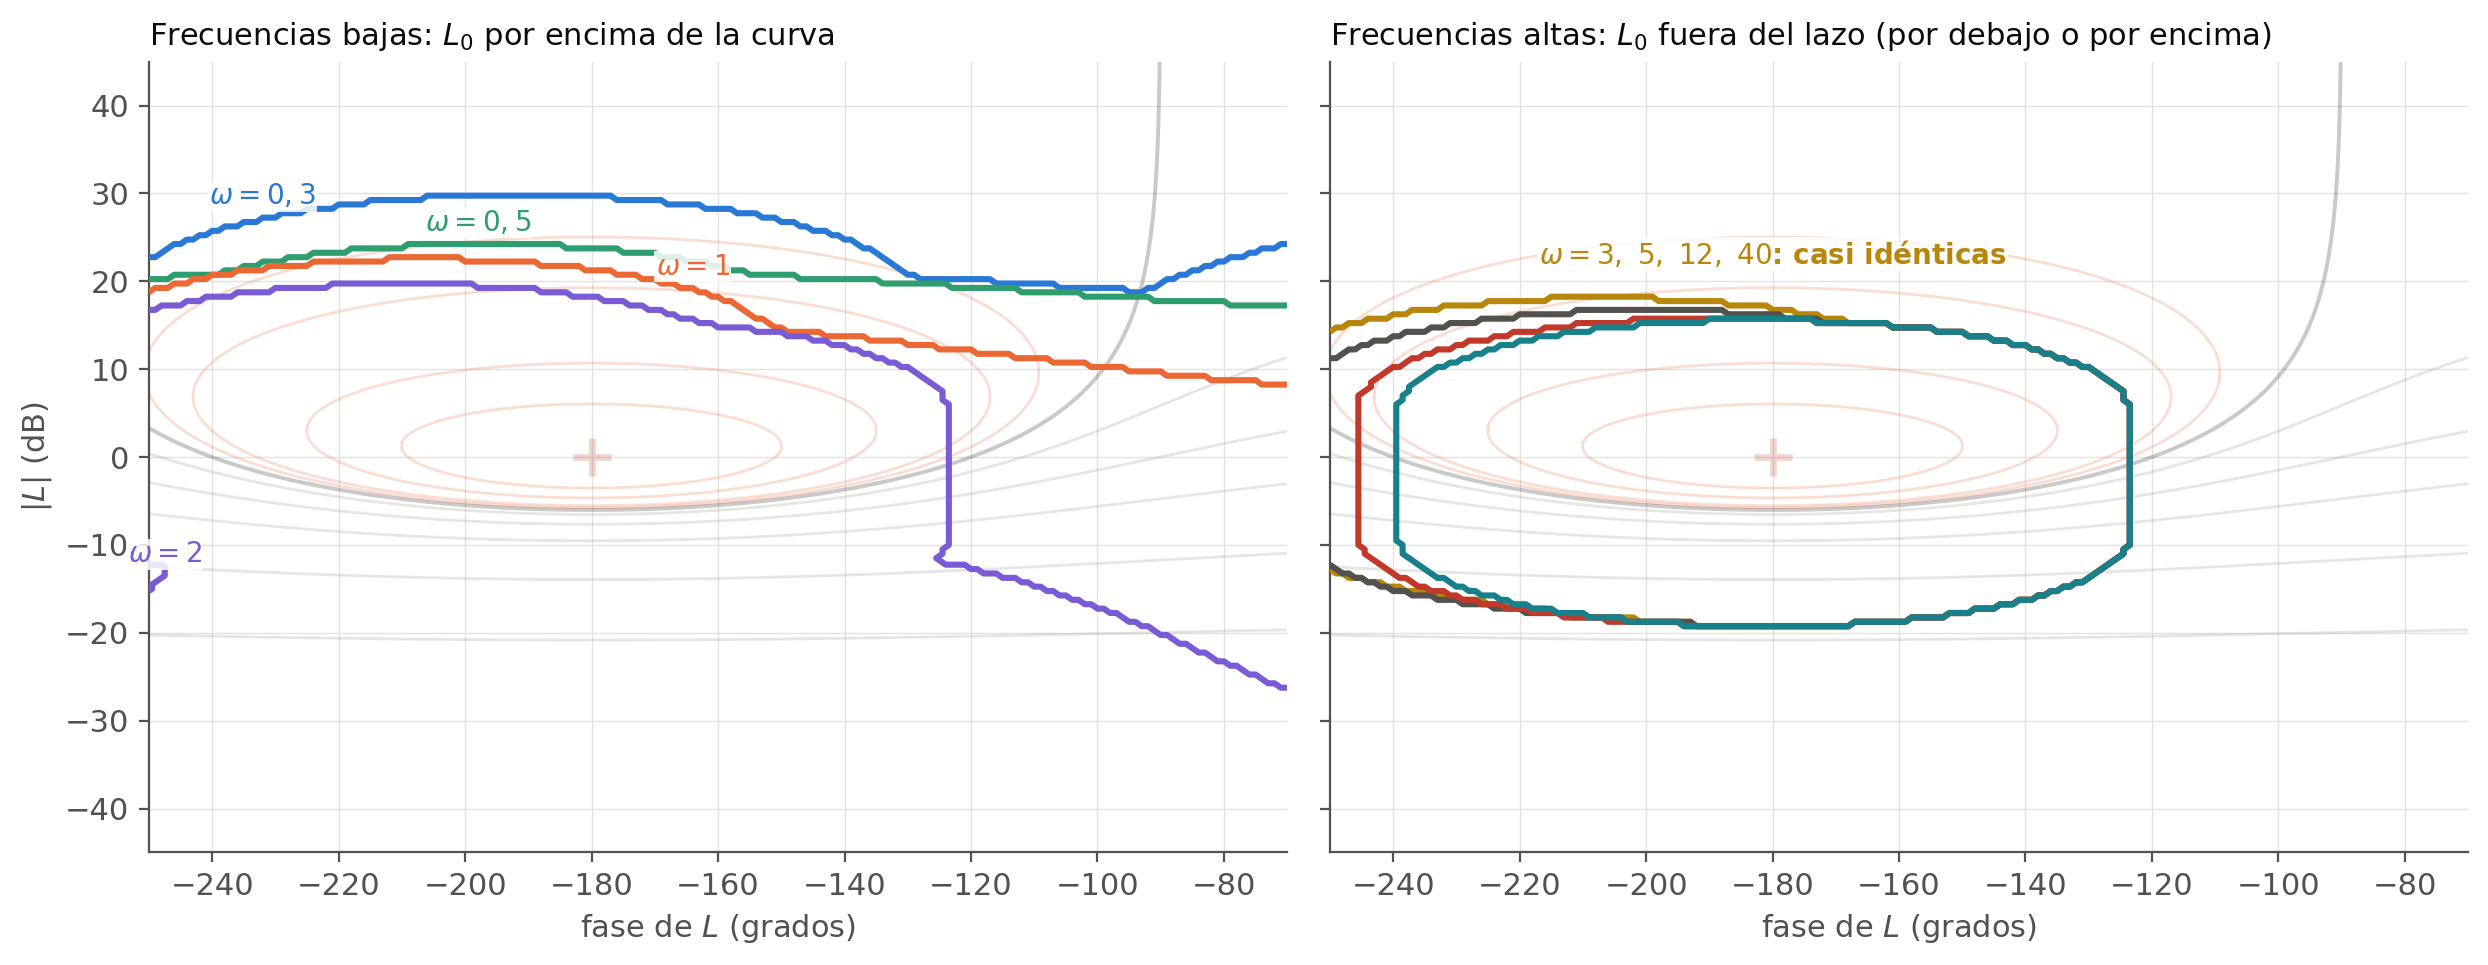
\includegraphics[width=0.95\textwidth]{fig/bounds.png}\\[2pt]
  \begin{columns}[T]
  \begin{column}{0.48\textwidth}
    \textbf{Bajas $\omega$} ($0.3$ a $2$): la curva es una especie de ``techo''. El nominal debe quedar \emph{por encima}: mucha ganancia ($\approx$ 20 a 30 dB).
  \end{column}
  \begin{column}{0.48\textwidth}
    \textbf{Altas $\omega$} ($\geq3$): un lazo cerrado alrededor del punto crítico. El nominal debe quedar \emph{fuera}: o muy arriba, o muy abajo ($\lesssim-19$ dB).
  \end{column}
  \end{columns}
\end{frame}

\begin{frame}{Cómo se usa un bound}
  \small
  \begin{block}{Regla}
    En cada frecuencia $\omega_i$, el punto $L_0(j\omega_i)$ debe quedar \textbf{del lado permitido} del bound de $\omega_i$.
  \end{block}
  \begin{itemize}
    \item $L_0(j\omega)=G(j\omega)P_0(j\omega)$ es una curva que recorre el mapa al variar $\omega$.
    \item Cada punto de la curva se compara con \emph{su} bound, no con los demás.
    \item $G$ mueve cada punto: sube/baja con su ganancia, desplaza en horizontal con su fase.
  \end{itemize}
  \begin{alertblock}{Paso 9}
    Elegir $G(s)$ hasta que todos los puntos $L_0(j\omega_i)$ queden en la zona buena.
  \end{alertblock}
\end{frame}

\begin{frame}{Ejercicio}
  \footnotesize
  A $\omega=2$ el nominal está en $L_0=3.16\angle-150^\circ$ ($10$ dB). Respecto al nominal, los otros puntos del template son:
  \begin{center}
  \begin{tabular}{c|c|c}
    $(K,a)$ & $\Delta$fase & $\Delta$dB\\\hline
    (1,1) & $0^\circ$ & $0$\\
    (1,3) & $+29.7^\circ$ & $-4.15$\\
    (5,1) & $0^\circ$ & $+13.98$\\
    (5,3) & $+29.7^\circ$ & $+9.83$
  \end{tabular}
  \end{center}
  \begin{enumerate}
    \item Calcula $|T|$ en dB para cada planta ($L_k=L_0\cdot$ cociente).
    \item ¿Se cumple $|T|\le1.58$ dB? ¿Qué planta es la peor?
    \item ¿Se cumple la variación de seguimiento ($\delta(2)=17.5$ dB)?
    \item ¿Cuántos dB hay que subir el nominal, como mínimo, para cumplir (bound a $-150^\circ$: $14$ dB)?
  \end{enumerate}
  \textbf{Pista:} $|T|=\dfrac{r}{\sqrt{1+2r\cos\theta+r^2}}$.\quad\textcolor{gray}{Solución en el apéndice.}
\end{frame}

\begin{frame}{El catálogo clásico de especificaciones}
  \small
  En la literatura de QFT (García-Sanz, 2005, tabla I) las especificaciones se agrupan en \textbf{cinco} cotas sobre funciones de transferencia en lazo cerrado:
  \begin{center}\footnotesize
  \begin{tabular}{lll}
    \hline
    Cota & Función & Qué limita\\
    \hline
    $T_1$ & $\dfrac{PG}{1+PG}$ & estabilidad robusta (y ruido a la salida)\\
    $T_2$ & $\dfrac{1}{1+PG}$ & perturbación a la salida de la planta\\
    $T_3$ & $\dfrac{P}{1+PG}$ & perturbación en la entrada de la planta\\
    $T_4$ & $\dfrac{G}{1+PG}$ & esfuerzo de control\\
    $T_5$ & $F\,\dfrac{PG}{1+PG}$ & seguimiento (entre $T_L$ y $T_U$)\\
    \hline
  \end{tabular}
  \end{center}
  \begin{itemize}
    \item Todas, para $P$ fija y fase $\varphi$ fija, son \textbf{desigualdades cuadráticas en la ganancia} $g=|G|$: $a g^2+bg+c\ge0$. De ahí sale el cálculo exacto del paso 16.
    \item Nosotros hemos trabajado con $T_1$ (estabilidad), $T_2$ (perturbación) y $T_5$ (seguimiento); $T_3$ y $T_4$ se tratan igual, solo cambian $a$, $b$ y $c$.
  \end{itemize}
\end{frame}

\begin{frame}{Resumen}
  \small
  \begin{itemize}
    \item Tres especificaciones: estabilidad ($|T|\le W_s$), seguimiento (banda $T_L$--$T_U$) y perturbación ($|S|\le W_d$), todas para todas las plantas.
    \item Un \textbf{bound} es el borde de las posiciones del nominal que cumplen la especificación para \emph{todo} el template.
    \item Se calcula deslizando el template por el mapa y comprobando.
    \item A bajas $\omega$ el bound exige ganancia; a altas, el nominal debe quedar fuera de un lazo alrededor del punto crítico.
    \item Siguiente: elegir $G$ para dejar $L_0(j\omega)$ del lado bueno en todas las frecuencias.
  \end{itemize}
\end{frame}

\appendix
\begin{frame}\centering\Large Apéndice\end{frame}

\begin{frame}{Solución del ejercicio}
  \footnotesize
  \begin{columns}[T]
  \begin{column}{0.58\textwidth}
    \textbf{1.} Con $|T|=\frac{r}{\sqrt{1+2r\cos\theta+r^2}}$:
    \begin{center}
    \begin{tabular}{c|c|c|c}
      $(K,a)$ & $r$ & $\theta$ & $|T|$ (dB)\\\hline
      (1,1) & $3.16$ & $-150^\circ$ & $2.58$\\
      (1,3) & $1.96$ & $-120.3^\circ$ & $1.27$\\
      (5,1) & $15.8$ & $-150^\circ$ & $0.48$\\
      (5,3) & $9.81$ & $-120.3^\circ$ & $0.42$
    \end{tabular}
    \end{center}
    \textbf{2.} No: $2.58>1.58$ dB. La peor es (1,1), la de menor ganancia (esquina del nominal).\\[2pt]
    \textbf{3.} Sí: la variación es $2.58-0.42=2.16$ dB $\le17.5$ dB.\\[2pt]
    \textbf{4.} Por encima de $14$ dB a $-150^\circ$: hay que subir al menos $4$ dB.
  \end{column}
  \begin{column}{0.4\textwidth}
    \begin{block}{Qué especificación manda}
      A esta frecuencia y fase, la de \textbf{estabilidad}: el seguimiento sobra ($2.2\ll17.5$).
    \end{block}
  \end{column}
  \end{columns}
\end{frame}

\begin{frame}{Para curiosos: otras especificaciones que se tratan igual}
  \small
  \begin{itemize}
    \item \textbf{Ruido y esfuerzo de control:} $\left|\dfrac{G}{1+L}\right|\le W_n(\omega)$. Limita la ganancia de $G$ a alta frecuencia.
    \item \textbf{Perturbación en la entrada de la planta:} $\left|\dfrac{P}{1+L}\right|\le W_{di}(\omega)$.
    \item \textbf{Margen de ganancia y fase} explícitos: se traducen en contornos de $|T|$ o $|S|$.
  \end{itemize}
  \begin{block}{Siempre el mismo método}
    Escribir la especificación como una condición sobre $L_k=L_0\cdot P_k/P_0$, para todo $k$, deslizar el template y marcar el borde.
  \end{block}
\end{frame}
\end{document}
